\section{Założenia techniczne}
\label{sec:zalozenia_techniczne}

Ze względu na charakter aplikacji, jakim jest edukacyjna gra komputerowa,
opierająca się w dużym stopniu na renderowaniu grafiki,
do wykonania projektu wybrano silnik Unity w wersji 6000.0.25f1~\cite{unity_site}.
Z wielu zalet silnika Unity, kluczowe dla niniejszego projektu są:

\begin{citemize}
    \item Wsparcie dla wielu platform --
    Unity pozwala na tworzenie aplikacji na wiele platform jednocześnie, w tym przede wszystkim na systemy Windows, Linux oraz macOS.
    \item Prostota tworzenia aplikacji graficznych --
    Unity oferuje wiele narzędzi, które ułatwiają tworzenie interaktywnych aplikacji graficznych,
    dzięki czemu można skupić się na tworzeniu mechanik gry.
    \item Szerokie wsparcie --
    Unity posiada rozbudowaną dokumentację~\cite{unity_docs},
    aktywne forum~\cite{unity_forum} oraz wiele darmowych zasobów.
\end{citemize}


Unity korzysta z języka C\#,
który bazuje na paradygmacie programowania obiektowego (ang. OOP — Object-Oriented Programming).
OOP opiera się na definiowaniu klas jako abstrakcji oraz tworzeniu ich instancji,
a także na współpracy między nimi~\cite{nygaard1986basic}.
Dzięki temu można tworzyć obiekty o wspólnych cechach,
co znacząco upraszcza pisanie kodu i jego późniejszą konserwację.\\
%Unity korzysta z języka C\#, opartego o paradygmat programowania obiektowego (ang. OOP -- Object-Oriented Programming),
%polegający na tworzeniu obiektów na podstawie abstrakcji klas, a także innych obiektów~\cite{nygaard1986basic}.
%Pozwala to na tworzenie wielu obiektów o podobnych cechach, co ułatwia pisanie kodu oraz jego późniejsze utrzymanie.\\
\indent Programowanie w silniku Unity opiera się na tzw. \textit{MonoBehaviour},
który jest klasą bazową dla większości skryptów w Unity.
Klasa ta pozwala na dostęp do informacji, jakie zawiera \textit{GameObject} oraz jego komponentów.
\textit{GameObject} jest natomiast Unitowym odpowiednikiem obiektu w edytorze,
składają się na niego komponenty, które odpowiadają za różne funkcje, jakie on pełni,
w tym przede wszystkim \textit{Transform}, który wskazuje pozycję, rotację oraz skalę obiektu.\\
\indent Kolejnym istotnym elementem w Unity są sceny,
które pozwalają na posiadanie wielu kilku różnych środowisk w jednym projekcie.
Sceny te mogą być wykorzystane do okna startowego oraz okna edytora schematu.
Resztę elementów można wykonać jako odrębne okienka w interfejsie użytkownika w danej scenie.
Wygląd edytora Unity przedstawiono na rys.~\ref{fig:unity_editor}.

\begin{figure}[h]
    \centering
    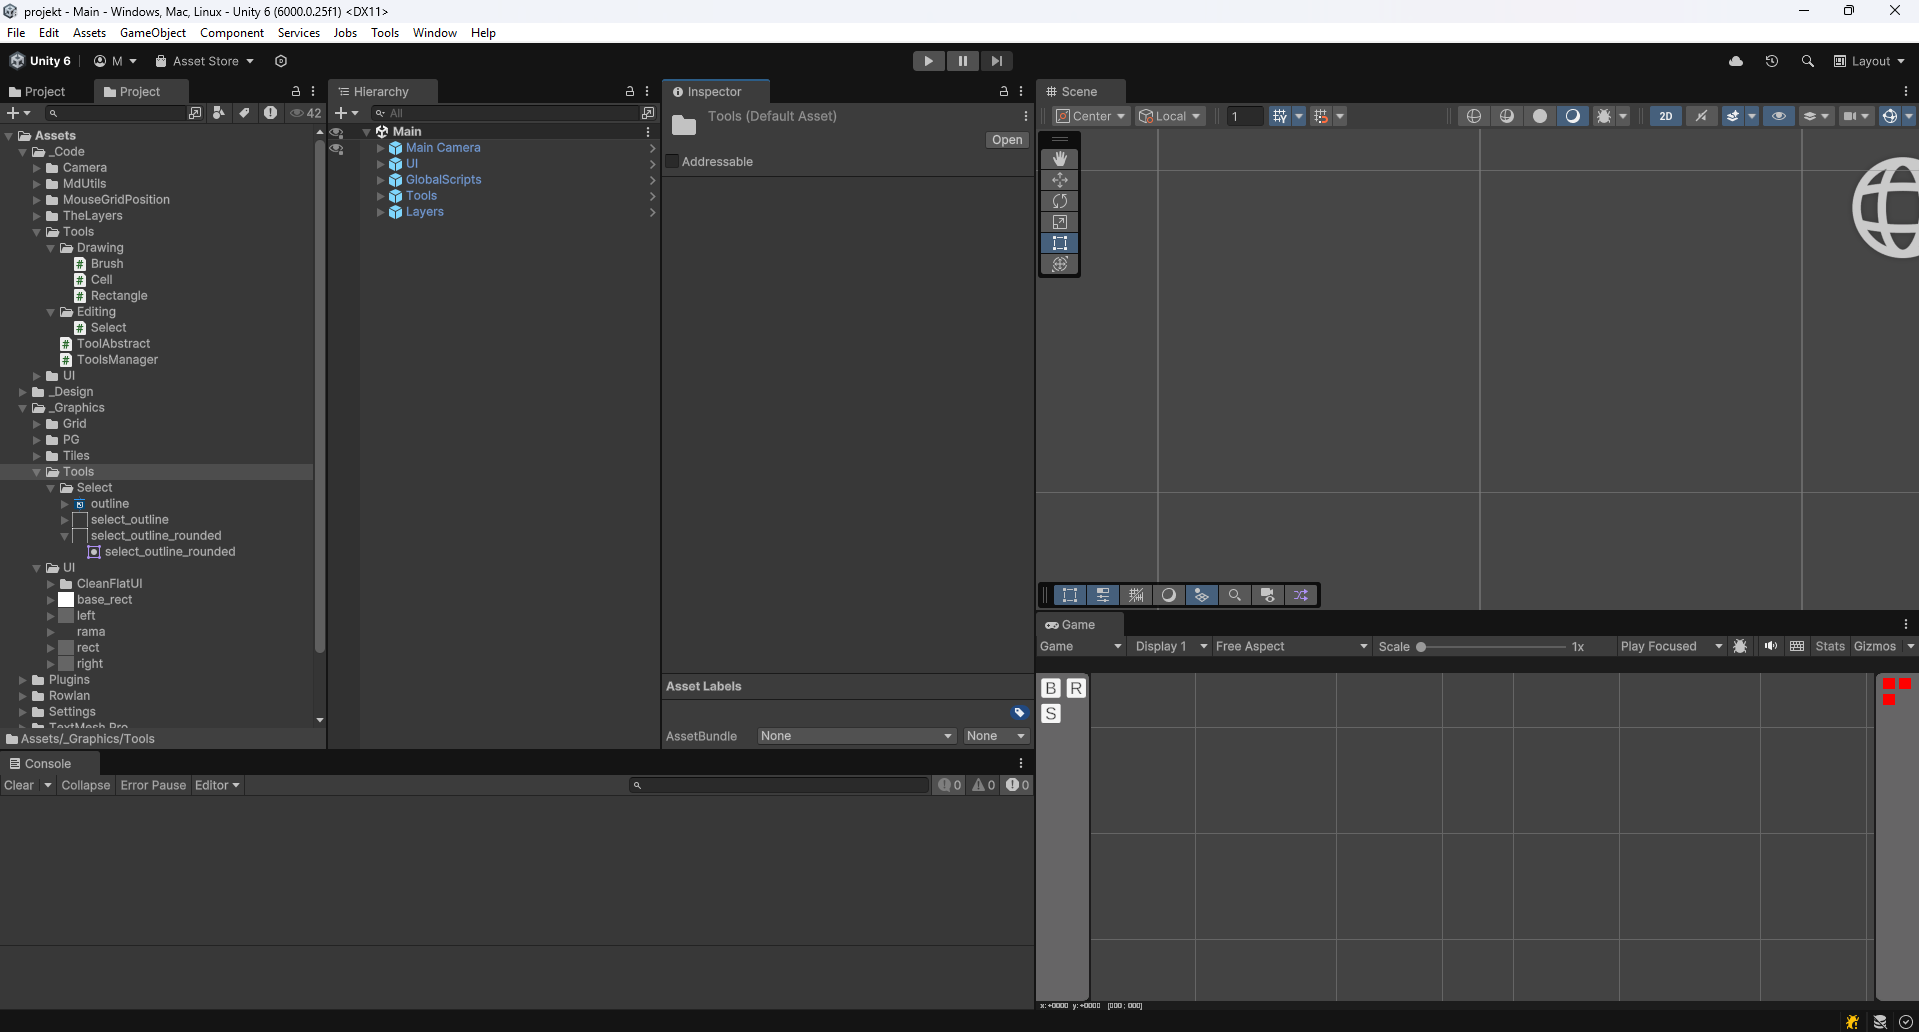
\includegraphics[width=0.9\textwidth]{chapters/chapter3/rys/unity_editor}
    \caption[Widok okna edytora Unity]{Wygląd edytora Unity, źródło: \cite{unity_site}}
    \label{fig:unity_editor}
\end{figure}

\subsection{Architektura programu}
\label{subsec:architektura_programu}

Aby zapewnić modularność oraz separację elementów aplikacji,
wykorzystano odpowiednio zaadaptowana architekturę MVVM (ang. Model-View-ViewModel).
Polega ona na podziale na trzy główne części: model, widok oraz widok-model.
Funkcje każdego z nich opisano w tab.~\ref{tab:mvvm}.

\begin{table}[h]
    \centering
    \caption[Opis funkcji poszczególnych elementów architektury MVVM.]
    {Opis funkcji poszczególnych elementów architektury MVVM, źródło:~\cite{mvvm}.}
    \label{tab:mvvm}
    \begin{tabular}{|c|p{0.6\textwidth}|}
        \hline
        Element & Opis \\
        \hline
        \hline
        Widok & Odpowiada za prezentację danych oraz interakcję z użytkownikiem. \\
        \hline
        Widok-model & Odpowiada za przekazywanie danych pomiędzy modelem a widokiem. \\
        \hline
        Model & Odpowiada za przechowywanie danych oraz logikę danego komponentu programu. \\
        \hline
    \end{tabular}
\end{table}

%Tak jak pierwotnie w architekturze MVVM,
%widok odpowiada za prezentację danych oraz interakcję z użytkownikiem.
%Przy czym po adaptacji widok-model odpowiada za nie tylko przekazywanie danych nie tylko między modelem a widokiem,
%ale również pomiędzy innymi częściami aplikacji jako menedżer danego systemu aplikacji.
%Sam model natomiast składa się z wielu komponentów, które przechowują dane oraz logikę danego komponentu aplikacji.
Przy większych projektach model ten jest stosowany do większości komponentów składających się na aplikację.
Widok-model w tej sytuacji odpowiada za przekazywanie danych nie tylko między modelem a widokiem,
ale również pomiędzy innymi częściami wewnątrz aplikacji jako menedżer danego systemu.
W przypadku opracowywanego programu można wyróżnić cztery główne systemy dotyczące różnych aspektów aplikacji:

\begin{citemize}
    \item System zarządzania progresem gry, odpowiadający za kontrolę przebiegu gry,
    a także punktację oraz weryfikację poziomów,
    \item Narzędzia do rysowania i edycji, wybieranie ich oraz kontrola ich działania,
    \item System zarządzania rysowanym schematem,
    odpowiadający za renderowanie warstw i przechowywanie informacji o nich
    oraz kontrolujący ich widok czy połączenia, na jakie się składają,
    \item System zapisu, odpowiadający za zapis i odczyt stanu gry.
\end{citemize}

%zarządzanie progresem gry, narzędzia do rysowania i edycji, system zarządzania rysowanym schematem, oraz system zapisu.
Odstępstwem od architektury MVVM jest natomiast potrzeba bezpośredniej interakcji pomiędzy użytkownikiem
a narzędziami ze względu na ich różnorodność, co przekłada się także na mniej skomplikowany kod.\\
Zarys architektury programu przedstawiono na rys.~\ref{fig:architektura}.

\begin{figure}[h!]
    \centering
    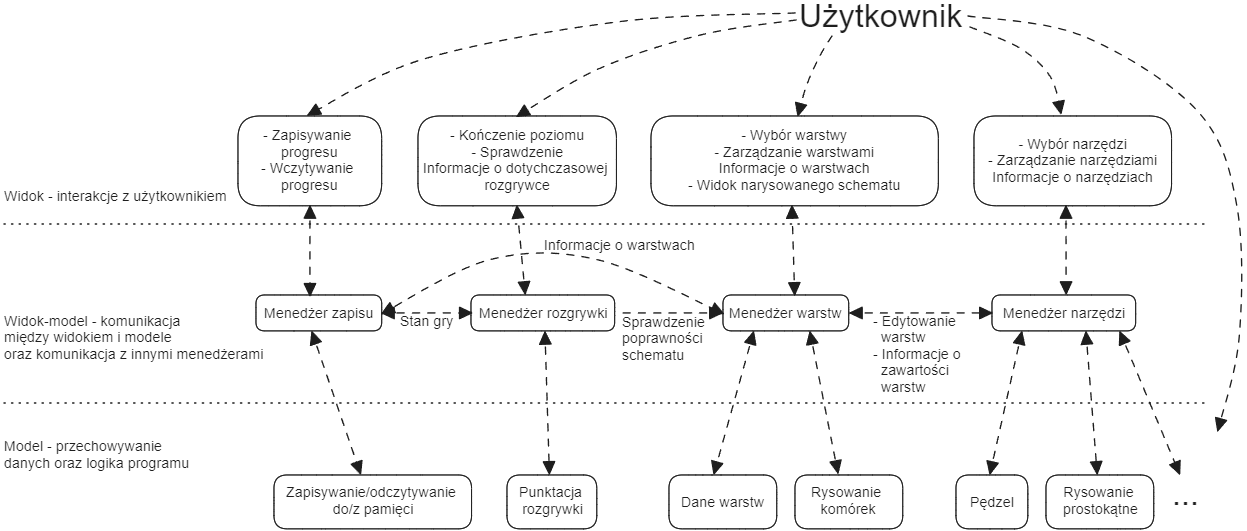
\includegraphics[width=\textwidth]{chapters/chapter3/rys/arch}
    \caption[Architektura programu.]{Architektura programu, źródło: opracowanie własne.}
    \label{fig:architektura}
\end{figure}

%\newpage % TODO: check this if something changes
\subsection{Wykorzystanie funkcji Unity oraz paczek zasobów}
\label{subsec:zasoby}

Do rysowania komórek schematów wykorzystano komponent \textit{SpriteRenderer},
pozwalający na renderowanie dwu-wymiarowych obrazów nazywanych \textit{sprite'ami}.
Dużą zaletą tego komponentu jest wbudowana optymalizacja ze strony Unity.
Obiektów tego typu może być wiele na scenie oraz są one renderowane tylko,
gdy są widoczne na ekranie~\cite{unity_csharp, unity_docs}. \\
\indent Prócz podstawowego skryptu, na jakim bazuje Unity, czyli \textit{MonoBehaviour},
wykorzystano także \textit{ScriptableObject}.
Jest to klasa, która pozwala na tworzenie obiektów, które mogą przechowywać dane zdefiniowane poza pracą programu,
a nawet wykonywać prostą logikę~\cite{unity_csharp, unity_docs}.
%Pozwala to na szczególną modularność dzięki możliwości wcześniejszego zdefiniowania danych zawartych w obiekcie
%i co mają one robić, a następnie tworzenie obiektów na ich podstawie.
Działanie SO jest zbliżone do klas i obiektów w OOP,
przy czym SO jest wykorzystywany przede wszystkim w edytorze Unity.
Dzięki temu można wcześniej zdefiniować jaki rodzaj danych powinien przechowywać dany typ obiektu,
a następnie tworzyć na ich podstawie konkretne instancje, których dane można zmieniać w edytorze.
Zostało to w szczególności wykorzystane w systemach zarządzania, rysowanym schematem
i narzędziami do rysowania i edycji.\\
%W przypadku schematu SO przechowuje informacje o tym jak powinny wyglądać i zachowywać się warstwy,
%natomiast do narzędzi SO zostały wykorzystane jako konfiguracje 
\indent W celu optymalizacji wskazane jest korzystanie z asynchroniczności w programie.
W szczególności jest to istotne podczas rysowania lub modyfikowania większych obszarów,
ponieważ wymaga to działania na wielu komórkach.
Skorzystano tutaj z paczki zasobów \textit{UniTask} do obsługi asynchroniczności,
dostępnej na platformie GitHub~\cite{unitask}.
Paczka ta adaptuje wbudowany w C\# system asynchroniczności,
dzięki czemu jest on znacznie optymalniejszy pod kątem wykorzystania w silniku Unity.


\subsection{Interfejs użytkownika}
\label{subsec:interfejs_uzytkownika}

Interfejs użytkownika (ang. \textit{User Interface}) jest jednym z kluczowych elementów każdej aplikacji,
kluczowe jest, aby był on intuicyjny oraz przejrzysty tak,
aby użytkownik mógł skupić się na korzystaniu z programu.
W przypadku opracowywanej aplikacji należy rozdzielić ją na dwie warstwy,
edytor schematów oraz część dotyczącą gry.
Jako że przez większość pracy w programie użytkownik ma do czynienia z edytorem schematów,
jest on podstawowym widokiem.
Z kolei elementy interfejsu dotyczące gry powinny być w formie nakładki na edytor schematów,
z wyjątkiem okna startowego, który będzie odrębną sceną, przez co nie ma potrzeby tworzenia nakładki.
Zarys widoku okna edytora schematów przedstawiono na rys.~\ref{fig:editor}.

\begin{figure}[h]
    \centering
    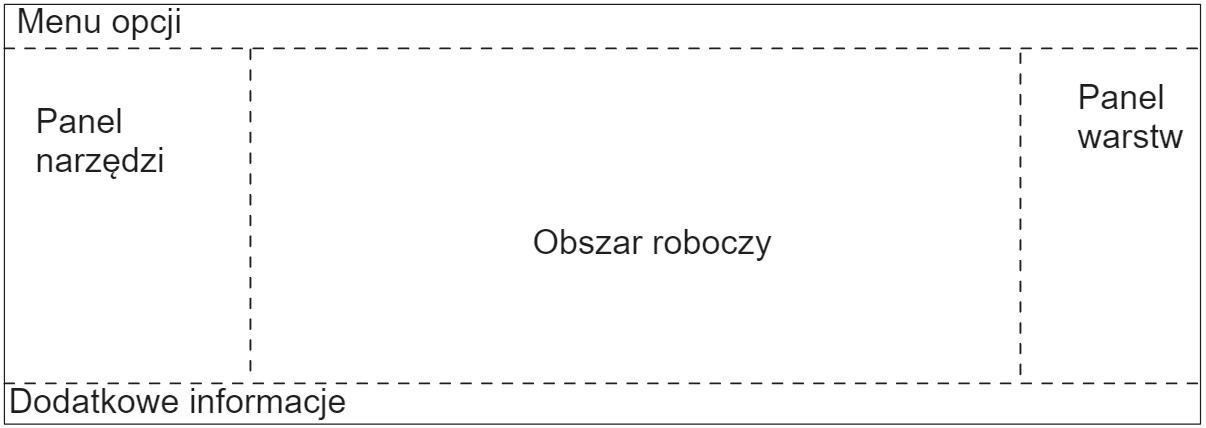
\includegraphics[width=0.89\textwidth]{chapters/chapter3/rys/ui_projekt}
    \caption[Szkic okna edytora schematów]{Szkic okna edytora schematów, źródło: opracowanie własne.}
    \label{fig:editor}
\end{figure}

\indent Okno dla edytora adaptuje elementy
z programów wspomnianych w rozdziale~\ref{ch:przeglad_istniejacych_rozwiazan}.
Tak jak w przypadku większości rozwiązań u góry okna znajduje się pasek opcji programu,
implementujący również opcje związane z grą.
Poniżej znajduje się obszar roboczy, gdzie użytkownik może rysować schematy.
Na dole okna znajduje się pasek informacyjny, który zawiera dane o aktualnie wybranym narzędziu,
a także o możliwych dodatkowych akcjach do wykonania.
Z prawej strony okna znajduje się panel warstw, zawierający dostępne warstwy schematu,
a także dodatkowe informacje o nich wraz z możliwością wyłączenia ich widoczności.
Po lewej usytuowany jest panel narzędzi, zawierający dostępne funkcje rysowania i edycji schematów
i dostępne dla nich opcje.
